\section{Manufactured solutions}
\subsection{Exact 1D solution}
A simple 1D square or plug wave should propagate witth exact plug shape when $c\Delta t\Delta x = 1$. We choose c = 1, and set $\Delta t = \Delta x$, and 
use a plug as our inital condition. The plug splits in half and the two parts propagates in opposite direction as seen in figure (\ref{fig_plug}).

\begin{figure}[H]
 \subfigure[Plug picture 0]{
\includegraphics[width=0.4\textwidth]{plog0000.png}}
 \subfigure[Plug picture 1]{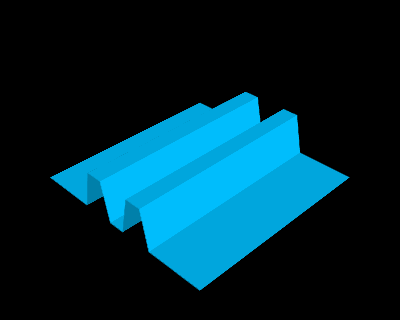
\includegraphics[width=0.4\textwidth]{plog0001.png}}
 \subfigure[Plug picture 2]{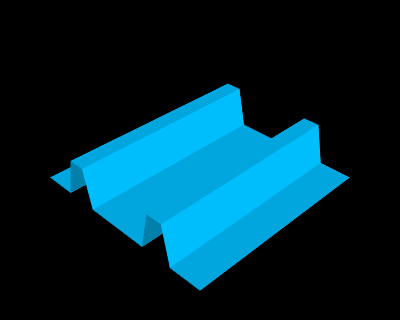
\includegraphics[width=0.4\textwidth]{plog0002.png}}
 \subfigure[Plug picture 3]{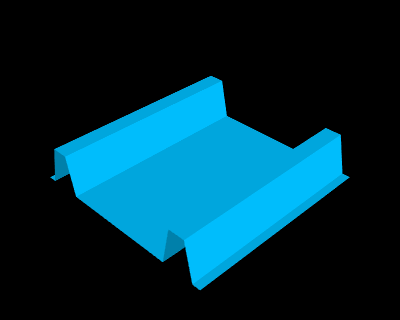
\includegraphics[width=0.4\textwidth]{plog0003.png}}
 \subfigure[Plug picture 4]{
\includegraphics[width=0.4\textwidth]{plog0004.png}}
 \subfigure[Plug picture 5]{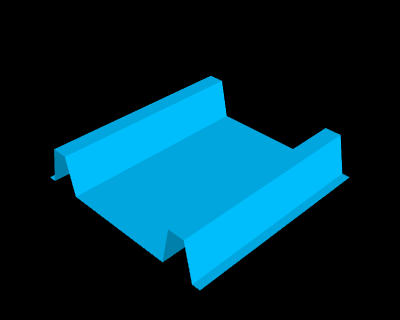
\includegraphics[width=0.4\textwidth]{plog0005.png}}
 \caption{The plug shape wave - first 6 pictures of a movie called plug.gif}
 \label{fig_plug}
 
\end{figure}

We see that the plug propagates exactly how we wanted it to. The movie of the plug has the name plug.gif.

\subsection{Standing wave}
As a test of the program, we manufactured a solution for constant q (this means that the velocity of the waves is constant over the domain). The wanted solution
is a standing wave given in eq. (\ref{standing_wave}).
\begin{equation}
 u(x,y,t) = e^{-bt} \cos(\frac{m_x \pi}{L_x}) \cos(\frac{m_y \pi}{L_y}) \cos(\omega t)
 \label{standing_wave}
\end{equation}
$m_x$ and $m_y$ are arbitrary integers that decides how many wavetops we end up with on our domain. The parameter $\omega$
is the frequency, and has to be chosen to fit the numerical solution.\\
To manufactor this solution we start by letting the initial condition be the exact standing wave at a time t=0. We need to fit the source term f(x,y,t) so that eq. (\ref{standing_wave})
is a solution to our wave equation (eq. \ref{wave_eq}), and find a suitable initial velocity V(x,y). 


\subsubsection{Finding f(x,y,t)}
Choose some $q(x,y) = A$ , $A \neq 0$ eq.(\ref{wave_eq}) becomes

\begin{equation}
 \frac{\partial^2 u}{\partial t^2} + v \frac{\partial u}{\partial t} = A \frac{\partial^2 u}{\partial x^2} + \frac{\partial^2 u}{\partial y^2} +f(x,y,t) 
\label{mod_wave_eq}
 \end{equation}



If we now insert eq.(\ref{standing_wave}) into eq.(\ref{mod_wave_eq}) we get

\begin{align*}
 \frac{\partial u}{\partial t} &= - b u(x,y,t) - \omega \underbrace{\frac{\sin(\omega t)}{\cos(\omega t)}}_{\tan(\omega t)}u(x,y,t) \\
 \frac{\partial^2 u}{\partial t^2} &= (b^2 -\omega^2) u(x,y,t) + 2\omega b \underbrace{\frac{\sin(\omega t)}{\cos(\omega t)}}_{\tan(\omega t)}u(x,y,t) \\
 \frac{\partial^2 u}{\partial x^2} &= - \left( \frac{m_x \pi}{L_x} \right)^2 u(x,y,t) \\
 \frac{\partial^2 u}{\partial y^2} &= - \left( \frac{m_y \pi}{L_y} \right)^2 u(x,y,t)
 \end{align*}
 
 \begin{align*}
  \Rightarrow \left[ (b^2 -\omega^2) + 2\omega b \tan(\omega t) - b^2 - b\omega \tan(\omega t) \right] u(x,y,t) = - A \left[ \left( \frac{m_x \pi}{L_x} \right)^2 + \left( \frac{m_y \pi}{L_y} \right)^2 \right] u(x,y,t) + f(x,y,t)\\
  \Rightarrow f(x,y,t) = \left[ \omega b \tan(\omega t) - \omega^2 + A \pi^2 \left( \left( \frac{m_x}{L_x} \right)^2 + \left( \frac{m_y}{L_y} \right)^2 \right) \right] u(x,y,t)
 \end{align*}
 So now we have our source term:
 \begin{equation}
  f(x,y,t) = \left[ \omega b \tan(\omega t) - \omega^2 + A \pi^2 \left( \left( \frac{m_x}{L_x} \right)^2 + \left( \frac{m_y}{L_y} \right)^2 \right) \right] u(x,y,t)
  \label{source}
 \end{equation}


\subsubsection{Finding V(x,y)}
The initial velocity is given by the exact solution (the initial condition) by
\begin{equation*}
 V(x,y) = \frac{\partial u(x,y,t)}{\partial t}|_{t=0}
\end{equation*}
We already found the time derivative of u in the latter subsection (finding f(x,y,t)),
\begin{equation}
 V(x,y) = \frac{\partial u(x,y,t)}{\partial t}|_{t=0} = -(\omega tan(\omega t) + b)u(x,y,t) |_{t=0} = -bu(x,y,t=0)
 \label{V_standing}
\end{equation}



\subsubsection{The results}
We have found all the expressions we need to implement the standing wave. Figure (\ref{exact_fig}) shows the initial condition (the exact solution at t=0).


\begin{figure}[H]
 \centering
 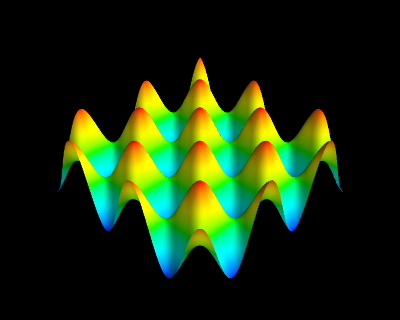
\includegraphics[width=0.5\textwidth]{u_exact1.png}
 \caption{The exact solution at t=0, also the initial condition}
 \label{exact_fig}
\end{figure}



\begin{figure}
 \subfigure[Exact standing wave]{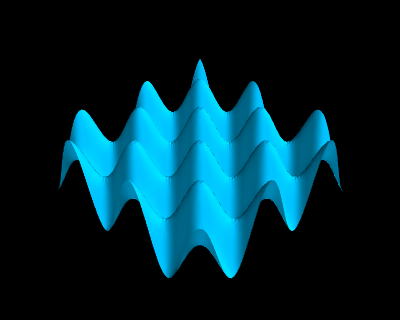
\includegraphics[width=0.4\textwidth]{exact0000.png}}
 \subfigure[Numerical standing wave]{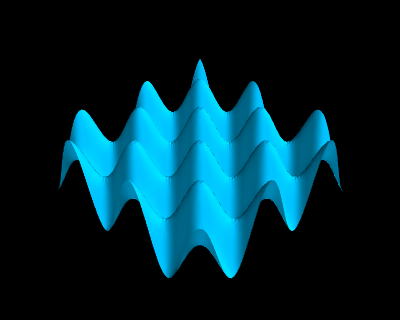
\includegraphics[width=0.4\textwidth]{num0000.png}}
 \subfigure[Exact standing wave]{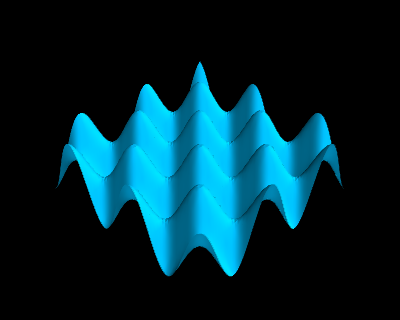
\includegraphics[width=0.4\textwidth]{exact0001.png}}
 \subfigure[Numerical standing wave]{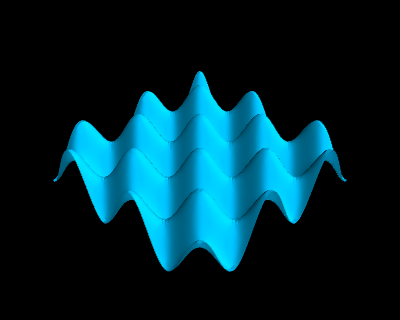
\includegraphics[width=0.4\textwidth]{num0001.png}}
 \subfigure[Exact standing wave]{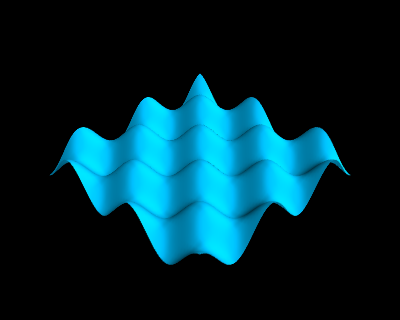
\includegraphics[width=0.4\textwidth]{exact0002.png}}
 \subfigure[Numerical standing wave]{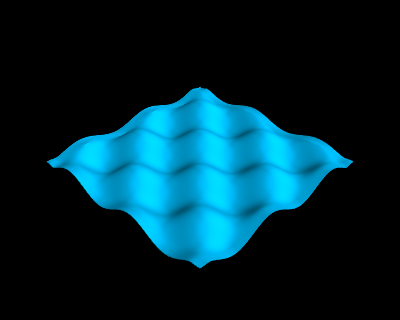
\includegraphics[width=0.4\textwidth]{num0002.png}}
 \subfigure[Exact standing wave]{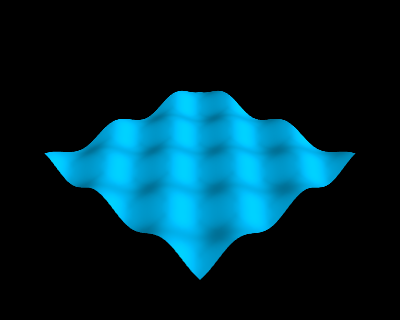
\includegraphics[width=0.4\textwidth]{exact0003.png}}
 \subfigure[Numerical standing wave]{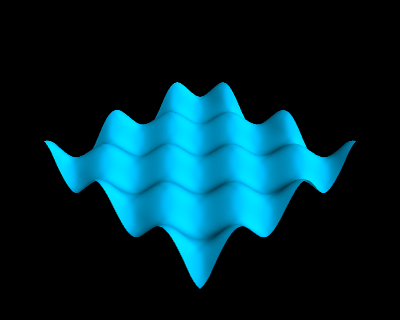
\includegraphics[width=0.4\textwidth]{num0003.png}}
\end{figure}

\begin{figure}
 \subfigure[Exact standing wave]{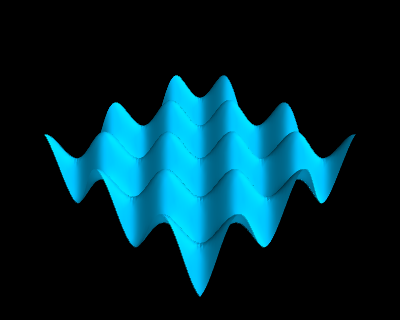
\includegraphics[width=0.4\textwidth]{exact0004.png}}
 \subfigure[Numerical standing wave]{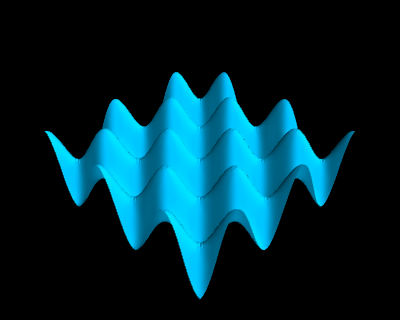
\includegraphics[width=0.4\textwidth]{num0004.png}}
 \subfigure[Exact standing wave]{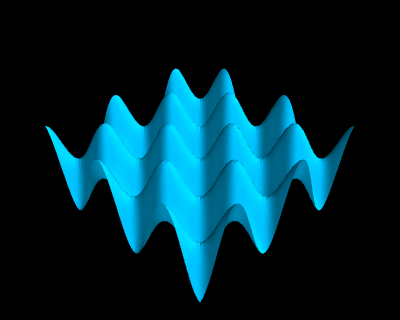
\includegraphics[width=0.4\textwidth]{exact0005.png}}
 \subfigure[Numerical standing wave]{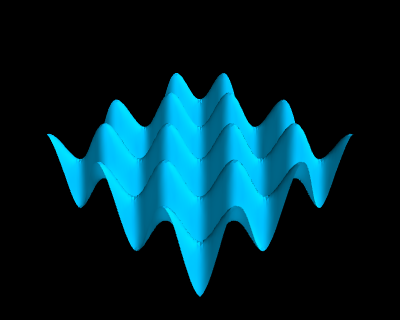
\includegraphics[width=0.4\textwidth]{num0005.png}}
 \label{fig_standing_num_exact}
 \caption{This is the first 6 pictures of two movies, one showing the exact solution and the other showing the numerically found solution.}
\end{figure}

Figure (\ref{fig_standing_num_exact}) is the first 6 pictures of two movies (FYLL INN NAVN PÅ FILMENE), where one shows the exact solution and the other shows the
numerical solution. The numerically found solution looks good when you look at that movie alone, but when you compare it to the exact solution you see that
it is a bit off. Picture (e),(f),(g) and (h) are typical examples of the difference between the numerical and exact solution. This is not very good, so lets analyse the results.\\
The error E is assumed to behave like
\begin{equation}
 E = C_t \Delta t^2 + C_x \Delta x^2 + C_y \Delta y^2
\end{equation}
choose $\Delta t = F_th$, $\Delta x = F_x h$ and $\Delta y = F_y h$, where $F_t,F_x,F_y$ are freely chosen constants factors compatible with the stability criterion.
The error can then be expressed as
\begin{equation}
 E = Ch^2
\end{equation}
where $C = C_xF_t^2 + C_yF_x^2 + C_tF_t^2$. This means that $E/h^2$ should be approximately constant.\\
We chose $F_t=1$, meaning $h = \Delta t$. The stability criterion says that $\Delta x = \Delta t \sqrt{2} = h\sqrt{2} \Rightarrow F_x = \sqrt{2}$.
The same argumentation give $F_y = \sqrt{2}$. Our program automaticly sets $\Delta x = \Delta t\sqrt{2}$ and $\Delta y = \Delta t \sqrt{2}$, so all we need to do
is run the program for different $\Delta t$ and see how the error behaves. Below is the results of our analysis

\begin{verbatim}
error for dt=1.00: 2.7598 
E/h**2: 2.7598 
error for dt=0.50: 0.7953 
E/h**2: 3.1810 
error for dt=0.20: 0.5349 
E/h**2: 13.3727 
error for dt=0.10: 0.2529 
E/h**2: 25.2943 
error for dt=0.02: 0.2987 
E/h**2: 746.7569 
error for dt=0.01: 0.3175 
E/h**2: 3175.3953 
\end{verbatim}

The absolute error decreases from $\Delta t = 1$ to $\Delta t = 0.02$, and after that it starts increasing again. We see that $E/h^2$ is clearly not 
constant, it increases fast as $\Delta t$ decreases. This tells us something is wrong with our program, and we have spendt many hours trying to find 
the source of this error, unsuccesfully. 






